%%%%%%%%%%%%%%%%%%%%%%%%%%%%%%%%%%%%%%%%%
% Beamer Presentation
% LaTeX Template
% Version 1.0 (10/11/12)
%
% This template has been downloaded from:
% http://www.LaTeXTemplates.com
%
% License:
% CC BY-NC-SA 3.0 (http://creativecommons.org/licenses/by-nc-sa/3.0/)
%
%%%%%%%%%%%%%%%%%%%%%%%%%%%%%%%%%%%%%%%%%


%% ist Essen, welches Mitpatienten übriglassen
%% versteckt häufig Schnüre und Gürtel (V.a. auf Vorbereitung zur Strangulation)
%% Paranoider, Schuldwahn und Verarmungswahn. 

%----------------------------------------------------------------------------------------
%	PACKAGES AND THEMES
%----------------------------------------------------------------------------------------

\documentclass{beamer}

\mode<presentation> {

% The Beamer class comes with a number of default slide themes
% which change the colors and layouts of slides. Below this is a list
% of all the themes, uncomment each in turn to see what they look like.

\usetheme{default}
%\usetheme{AnnArbor}
%\usetheme{Antibes}
%\usetheme{Bergen}
%\usetheme{Berkeley}
%\usetheme{Berlin}
%\usetheme{Boadilla}
%\usetheme{CambridgeUS}
%\usetheme{Copenhagen}
%\usetheme{Darmstadt}
%\usetheme{Dresden}
%\usetheme{Frankfurt}
%\usetheme{Goettingen}
%\usetheme{Hannover}
%\usetheme{Ilmenau}
%\usetheme{JuanLesPins}
%\usetheme{Luebeck}
%\usetheme{Madrid}
%\usetheme{Malmoe}
%\usetheme{Marburg}
\usetheme{Montpellier}
%\usetheme{PaloAlto}
%\usetheme{Pittsburgh}
%\usetheme{Rochester}
%\usetheme{Singapore}
%\usetheme{Szeged}
%\usetheme{Warsaw}

% As well as themes, the Beamer class has a number of color themes
% for any slide theme. Uncomment each of these in turn to see how it
% changes the colors of your current slide theme.

%\usecolortheme{albatross}
%\usecolortheme{beaver}
%\usecolortheme{beetle}
%\usecolortheme{crane}
%\usecolortheme{dolphin}
%\usecolortheme{dove}
%\usecolortheme{fly}
%\usecolortheme{lily}
%\usecolortheme{orchid}
%\usecolortheme{rose}
%\usecolortheme{seagull}
%\usecolortheme{seahorse}
%\usecolortheme{whale}
%\usecolortheme{wolverine}

%\setbeamertemplate{footline} % To remove the footer line in all slides uncomment this line
%\setbeamertemplate{footline}[page number] % To replace the footer line in all slides with a simple slide count uncomment this line

\setbeamertemplate{navigation symbols}{} % To remove the navigation symbols from the bottom of all slides uncomment this line
\setbeamertemplate{caption}[numbered]
}

%\usepackage{subfigure}
\usepackage{graphicx} % Allows including images
\usepackage{booktabs} % Allows the use of \toprule, \midrule and \bottomrule in tables
\usepackage[utf8]{inputenc}
\usepackage{helvet}
\usepackage{mathtools}
\usepackage{amsmath}
%\usepackage[font={small,it}]{caption}
\usepackage[skip=2pt, font=footnotesize]{caption}
\usepackage{ragged2e}
\usepackage{epstopdf}
\usepackage{svg}
\usepackage[sort,round]{natbib}
\bibliographystyle{authordate1}
\usepackage{tikz}

\usepackage{scrextend}
\changefontsizes{7.5pt}
%----------------------------------------------------------------------------------------
%	TITLE PAGE
%----------------------------------------------------------------------------------------

\title [Fallvorstellung 24.10.2017]{Fall X: Titel} % The short title appears at the bottom of every slide, the full title is only on the title page

\author{Veith Weilnhammer} % Your name
\institute[CCM] % Your institution as it will appear on the bottom of every slide, may be shorthand to save space
{Station 155

Klinik für Psychiatrie und Psychotherapie

Campus Charité Mitte

\medskip
{veith-andreas.weilnhammer@charite.de} % Your email address

\medskip

Behandler: XY
% Your institution for the title page



}

\date{}

\begin{document}


\begin{frame}
\titlepage % Print the title page as the first slide
\end{frame}



%----------------------------------------------------------------------------------------
%	PRESENTATION SLIDES
%----------------------------------------------------------------------------------------


%%%%%%%%%%%%%%%%
% Introduction
%%%%%%%%%%%%%%%%


%%%%%%%%%%%%%%%%
% Aufnahme
%%%%%%%%%%%%%%%%

\usebackgroundtemplate{%             declare it
\tikz[overlay,remember picture] \node[opacity=0.3, at=(current page.center)] {
   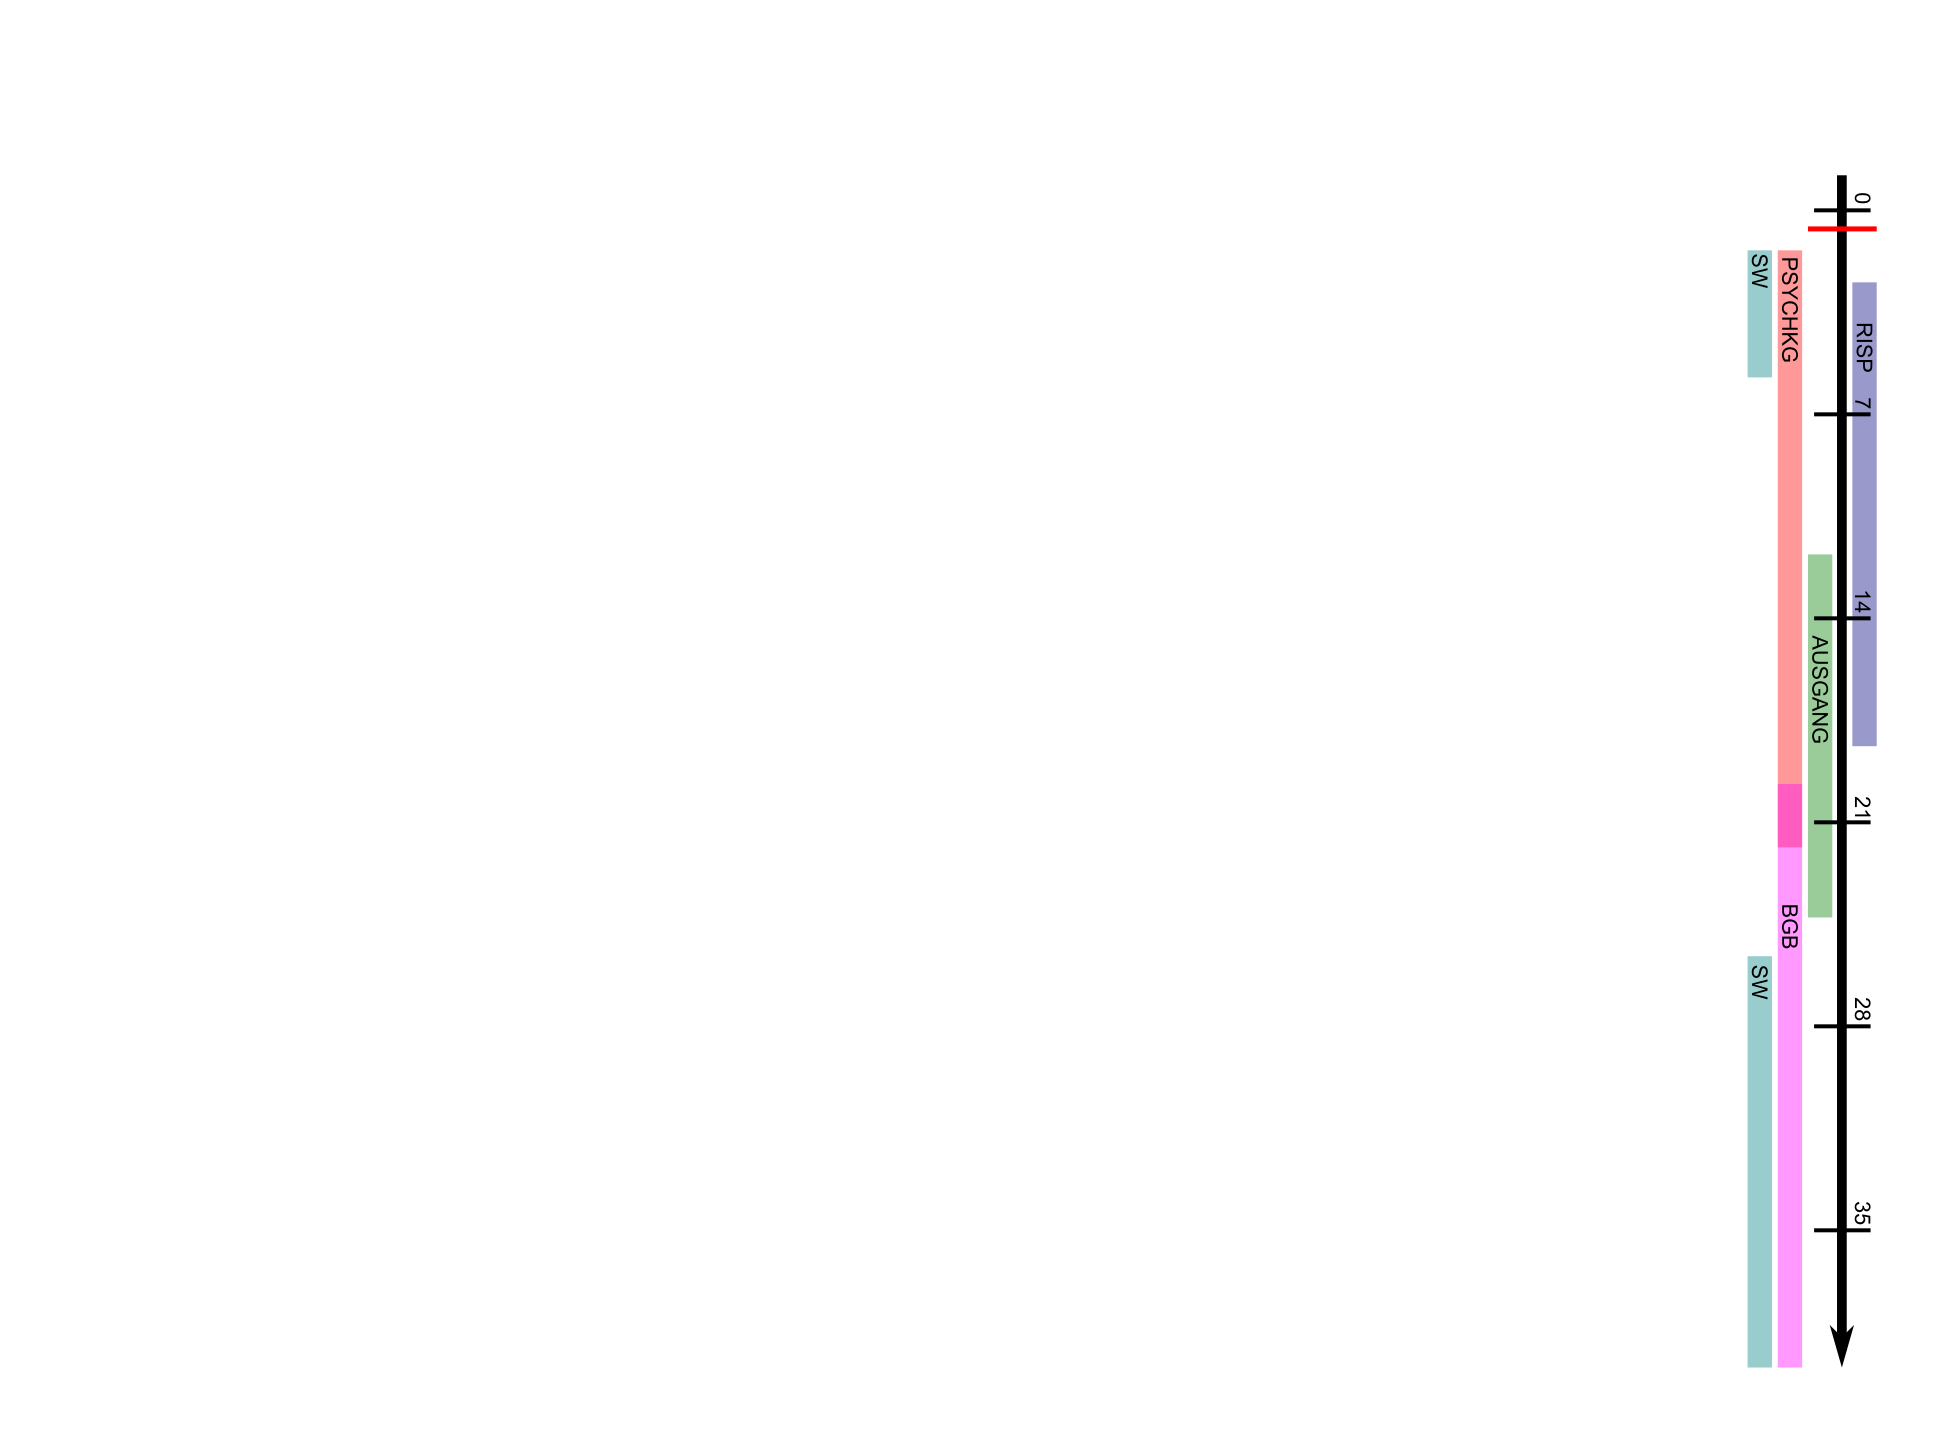
\includegraphics[height=0.95\paperheight,width=0.95\paperwidth]{d1.png}};
}

\section{Aufnahme}
\begin{frame}

%\frametitle{Anamnese 1}

 \begin{columns}[t] % The "c" option specifies centered vertical alignment while the "t" option is used for top vertical alignment
\column[T]{.9\textwidth} % Left column and width
 \vspace{0pt}
\begin{block}{Aktualanamnese}
\begin{itemize}
 \item \justifying XY
\end{itemize}
\end{block}

\begin{block}{PPB}
\begin{itemize}
\item \justifying XY
\end{itemize}
\end{block}

\begin{block}{Procedere}
\begin{itemize}
\item \justifying XY
\end{itemize}
\end{block}

\column[T]{.1\textwidth} % Right column and width

\end{columns}
\end{frame}



%%%%%%%%%%%%%%%%
% Verlauf
%%%%%%%%%%%%%%%%

\section{Behandlungsverlauf}


%%%%%%%%%%%%%%%%
% Verlauf
%%%%%%%%%%%%%%%%

\section{Therapiekonzept}

%%%%%%%%%%%%%%%%
% Diskussion
%%%%%%%%%%%%%%%%

\section{Diskussion}




%\begin{frame}
%\frametitle{Template}

 %\begin{columns}[t] % The "c" option specifies centered vertical alignment while the "t" option is used for top vertical alignment
%\column[T]{.9\textwidth} % Left column and width

%\column[T]{.1\textwidth} % Right column and width
 
%\end{columns}
%\end{frame}



\end{document} 